%&preformat-disser
\RequirePackage[l2tabu,orthodox]{nag} % Раскомментировав, можно в логе получать рекомендации относительно правильного использования пакетов и предупреждения об устаревших и нерекомендуемых пакетах
% Формат А4, 14pt (ГОСТ Р 7.0.11-2011, 5.3.6)
\documentclass[a4paper,12pt,oneside,openany]{memoir}

\input{common/setup}               % общие настройки шаблона
\input{common/packages}  % Пакеты общие для диссертации и автореферата
\synopsisfalse                           % Этот документ --- не автореферат
\input{Thesis/dispackages}         % Пакеты для диссертации
\usepackage{tabu, tabulary}  %таблицы с автоматически подбирающейся шириной столбцов
\usepackage{fr-longtable}    %ради \endlasthead

% Листинги с исходным кодом программ
\usepackage{fancyvrb}
\usepackage{listings}
\lccode`\~=0\relax %Без этого хака из-за особенностей пакета listings перестают работать конструкции с \MakeLowercase и т. п. в (xe|lua)latex

% Русская традиция начертания греческих букв
\usepackage{upgreek} % прямые греческие ради русской традиции

% Микротипографика
%\ifnumequal{\value{draft}}{0}{% Только если у нас режим чистовика
%    \usepackage[final]{microtype}[2016/05/14] % улучшает представление букв и слов в строках, может помочь при наличии отдельно висящих слов
%}{}

% Отметка о версии черновика на каждой странице
% Чтобы работало надо в своей локальной копии по инструкции
% https://www.ctan.org/pkg/gitinfo2 создать небходимые файлы в папке
% ./git/hooks
% If you’re familiar with tweaking git, you can probably work it out for
% yourself. If not, I suggest you follow these steps:
% 1. First, you need a git repository and working tree. For this example,
% let’s suppose that the root of the working tree is in ~/compsci
% 2. Copy the file post-xxx-sample.txt (which is in the same folder of
% your TEX distribution as this pdf) into the git hooks directory in your
% working copy. In our example case, you should end up with a file called
% ~/compsci/.git/hooks/post-checkout
% 3. If you’re using a unix-like system, don’t forget to make the file executable.
% Just how you do this is outside the scope of this manual, but one
% possible way is with commands such as this:
% chmod g+x post-checkout.
% 4. Test your setup with “git checkout master” (or another suitable branch
% name). This should generate copies of gitHeadInfo.gin in the directories
% you intended.
% 5. Now make two more copies of this file in the same directory (hooks),
% calling them post-commit and post-merge, and you’re done. As before,
% users of unix-like systems should ensure these files are marked as
% executable.
\ifnumequal{\value{draft}}{1}{% Черновик
   \IfFileExists{.git/gitHeadInfo.gin}{                                        
      \usepackage[mark,pcount]{gitinfo2}
      \renewcommand{\gitMark}{rev.\gitAbbrevHash\quad\gitCommitterEmail\quad\gitAuthorIsoDate}
      \renewcommand{\gitMarkFormat}{\rmfamily\color{Gray}\small\bfseries}
   }{}
}{}
\RequirePackage{natbib}
\RequirePackage{verbatim}
\RequirePackage{wrapfig}
\RequirePackage{float}        % Пакеты для специфических пользовательских задач

\input{Thesis/setup}               % Упрощённые настройки шаблона

\input{Thesis/preamblenames}       % Переопределение именований, чтобы можно было и в преамбуле использовать
\input{common/newnames}  % Новые переменные, которые могут использоваться во всём проекте

%%% Основные сведения %%%
\newcommand{\thesisAuthorLastName}{Кочуров}
\newcommand{\thesisAuthorOtherNames}{Максим Вадимович}
\newcommand{\thesisAuthorInitials}{М.В.}
\newcommand{\thesisAuthor}             % Диссертация, ФИО автора
{%
    \texorpdfstring{% \texorpdfstring takes two arguments and uses the first for (La)TeX and the second for pdf
        \thesisAuthorLastName~\thesisAuthorOtherNames% так будет отображаться на титульном листе или в тексте, где будет использоваться переменная
    }{%
        \thesisAuthorLastName, \thesisAuthorOtherNames% эта запись для свойств pdf-файла. В таком виде, если pdf будет обработан программами для сбора библиографических сведений, будет правильно представлена фамилия.
    }
}
\newcommand{\thesisAuthorShort}        % Диссертация, ФИО автора инициалами
{\thesisAuthorInitials~\thesisAuthorLastName}
%\newcommand{\thesisUdk}                % Диссертация, УДК
%{\todo{xxx.xxx}}
\newcommand{\thesisTitle}              % Диссертация, название
{Эконометрическое моделирование динамики корреляций доходностей финансовых стратегий}
\newcommand{\thesisSpecialtyNumber}    % Диссертация, специальность, номер
{38.03.01}
\newcommand{\thesisSpecialtyTitle}     % Диссертация, специальность, название
{Экономика}
\newcommand{\thesisDegree}             % Диссертация, ученая степень
{Бакалавр Экономики}
\newcommand{\thesisDegreeShort}        % Диссертация, ученая степень, краткая запись
{Бакалавр Экономики}
\newcommand{\thesisCity}               % Диссертация, город написания диссертации
{Москва}
\newcommand{\thesisYear}               % Диссертация, год написания диссертации
{2018}
\newcommand{\thesisOrganization}       % Диссертация, организация
{Московский государственный университет имени М.В.Ломоносова}
\newcommand{\thesisOrganizationShort}  % Диссертация, краткое название организации для доклада
{МГУ им. М.В.Ломоносова}

\newcommand{\thesisInOrganization}     % Диссертация, организация в предложном падеже: Работа выполнена в ...
{Московском государственном университете имени М.В.Ломоносова}

\newcommand{\supervisorFio}            % Научный руководитель, ФИО
{Лукаш Евгений Николаевич}
\newcommand{\supervisorRegalia}        % Научный руководитель, регалии
{доцент кандидат экономических наук}
\newcommand{\supervisorFioShort}       % Научный руководитель, ФИО
{Е.Н. Лукаш}
\newcommand{\supervisorRegaliaShort}   % Научный руководитель, регалии
{доцент к.э.н.}


\newcommand{\opponentOneFio}           % Оппонент 1, ФИО
{\todo{Фамилия Имя Отчество}}
\newcommand{\opponentOneRegalia}       % Оппонент 1, регалии
{\todo{доктор физико-математических наук, профессор}}
\newcommand{\opponentOneJobPlace}      % Оппонент 1, место работы
{\todo{Не очень длинное название для места работы}}
\newcommand{\opponentOneJobPost}       % Оппонент 1, должность
{\todo{старший научный сотрудник}}

\newcommand{\opponentTwoFio}           % Оппонент 2, ФИО
{\todo{Фамилия Имя Отчество}}
\newcommand{\opponentTwoRegalia}       % Оппонент 2, регалии
{\todo{кандидат физико-математических наук}}
\newcommand{\opponentTwoJobPlace}      % Оппонент 2, место работы
{\todo{Основное место работы c длинным длинным длинным длинным названием}}
\newcommand{\opponentTwoJobPost}       % Оппонент 2, должность
{\todo{старший научный сотрудник}}

\newcommand{\leadingOrganizationTitle} % Ведущая организация, дополнительные строки
{\todo{Федеральное государственное бюджетное образовательное учреждение высшего профессионального образования с~длинным длинным длинным длинным названием}}

\newcommand{\defenseDate}              % Защита, дата
{23 мая 2018~г.}
\newcommand{\defenseCouncilNumber}     % Защита, номер диссертационного совета
{\todo{Д\,123.456.78}}
\newcommand{\defenseCouncilTitle}      % Защита, учреждение диссертационного совета
{\todo{Название учреждения}}
\newcommand{\defenseCouncilAddress}    % Защита, адрес учреждение диссертационного совета
{\todo{Адрес}}
\newcommand{\defenseCouncilPhone}      % Телефон для справок
{\todo{+7~(0000)~00-00-00}}

\newcommand{\defenseSecretaryFio}      % Секретарь диссертационного совета, ФИО
{\todo{Фамилия Имя Отчество}}
\newcommand{\defenseSecretaryRegalia}  % Секретарь диссертационного совета, регалии
{\todo{д-р~физ.-мат. наук}}            % Для сокращений есть ГОСТы, например: ГОСТ Р 7.0.12-2011 + http://base.garant.ru/179724/#block_30000

\newcommand{\synopsisLibrary}          % Автореферат, название библиотеки
{\todo{Название библиотеки}}
\newcommand{\synopsisDate}             % Автореферат, дата рассылки
{\todo{DD mmmmmmmm YYYY года}}

% To avoid conflict with beamer class use \providecommand
\providecommand{\keywords}%            % Ключевые слова для метаданных PDF диссертации и автореферата
{}
      % Основные сведения
\input{common/styles}    % Стили общие для диссертации и автореферата
\input{Thesis/disstyles}           % Стили для диссертации
% для вертикального центрирования ячеек в tabulary
\def\zz{\ifx\[$\else\aftergroup\zzz\fi}
%$ \] % <-- чиним подсветку синтаксиса в некоторых редакторах
\def\zzz{\setbox0\lastbox
\dimen0\dimexpr\extrarowheight + \ht0-\dp0\relax
\setbox0\hbox{\raise-.5\dimen0\box0}%
\ht0=\dimexpr\ht0+\extrarowheight\relax
\dp0=\dimexpr\dp0+\extrarowheight\relax 
\box0
}



\lstdefinelanguage{Renhanced}%
{keywords={abbreviate,abline,abs,acos,acosh,action,add1,add,%
        aggregate,alias,Alias,alist,all,anova,any,aov,aperm,append,apply,%
        approx,approxfun,apropos,Arg,args,array,arrows,as,asin,asinh,%
        atan,atan2,atanh,attach,attr,attributes,autoload,autoloader,ave,%
        axis,backsolve,barplot,basename,besselI,besselJ,besselK,besselY,%
        beta,binomial,body,box,boxplot,break,browser,bug,builtins,bxp,by,%
        c,C,call,Call,case,cat,category,cbind,ceiling,character,char,%
        charmatch,check,chol,chol2inv,choose,chull,class,close,cm,codes,%
        coef,coefficients,co,col,colnames,colors,colours,commandArgs,%
        comment,complete,complex,conflicts,Conj,contents,contour,%
        contrasts,contr,control,helmert,contrib,convolve,cooks,coords,%
        distance,coplot,cor,cos,cosh,count,fields,cov,covratio,wt,CRAN,%
        create,crossprod,cummax,cummin,cumprod,cumsum,curve,cut,cycle,D,%
        data,dataentry,date,dbeta,dbinom,dcauchy,dchisq,de,debug,%
        debugger,Defunct,default,delay,delete,deltat,demo,de,density,%
        deparse,dependencies,Deprecated,deriv,description,detach,%
        dev2bitmap,dev,cur,deviance,off,prev,,dexp,df,dfbetas,dffits,%
        dgamma,dgeom,dget,dhyper,diag,diff,digamma,dim,dimnames,dir,%
        dirname,dlnorm,dlogis,dnbinom,dnchisq,dnorm,do,dotplot,double,%
        download,dpois,dput,drop,drop1,dsignrank,dt,dummy,dump,dunif,%
        duplicated,dweibull,dwilcox,dyn,edit,eff,effects,eigen,else,%
        emacs,end,environment,env,erase,eval,equal,evalq,example,exists,%
        exit,exp,expand,expression,External,extract,extractAIC,factor,%
        fail,family,fft,file,filled,find,fitted,fivenum,fix,floor,for,%
        For,formals,format,formatC,formula,Fortran,forwardsolve,frame,%
        frequency,ftable,ftable2table,function,gamma,Gamma,gammaCody,%
        gaussian,gc,gcinfo,gctorture,get,getenv,geterrmessage,getOption,%
        getwd,gl,glm,globalenv,gnome,GNOME,graphics,gray,grep,grey,grid,%
        gsub,hasTsp,hat,heat,help,hist,home,hsv,httpclient,I,identify,if,%
        ifelse,Im,image,\%in\%,index,influence,measures,inherits,install,%
        installed,integer,interaction,interactive,Internal,intersect,%
        inverse,invisible,IQR,is,jitter,kappa,kronecker,labels,lapply,%
        layout,lbeta,lchoose,lcm,legend,length,levels,lgamma,library,%
        licence,license,lines,list,lm,load,local,locator,log,log10,log1p,%
        log2,logical,loglin,lower,lowess,ls,lsfit,lsf,ls,machine,Machine,%
        mad,mahalanobis,make,link,margin,match,Math,matlines,mat,matplot,%
        matpoints,matrix,max,mean,median,memory,menu,merge,methods,min,%
        missing,Mod,mode,model,response,mosaicplot,mtext,mvfft,na,nan,%
        names,omit,nargs,nchar,ncol,NCOL,new,next,NextMethod,nextn,%
        nlevels,nlm,noquote,NotYetImplemented,NotYetUsed,nrow,NROW,null,%
        numeric,\%o\%,objects,offset,old,on,Ops,optim,optimise,optimize,%
        options,or,order,ordered,outer,package,packages,page,pairlist,%
        pairs,palette,panel,par,parent,parse,paste,path,pbeta,pbinom,%
        pcauchy,pchisq,pentagamma,persp,pexp,pf,pgamma,pgeom,phyper,pico,%
        pictex,piechart,Platform,plnorm,plogis,plot,pmatch,pmax,pmin,%
        pnbinom,pnchisq,pnorm,points,poisson,poly,polygon,polyroot,pos,%
        postscript,power,ppoints,ppois,predict,preplot,pretty,Primitive,%
        print,prmatrix,proc,prod,profile,proj,prompt,prop,provide,%
        psignrank,ps,pt,ptukey,punif,pweibull,pwilcox,q,qbeta,qbinom,%
        qcauchy,qchisq,qexp,qf,qgamma,qgeom,qhyper,qlnorm,qlogis,qnbinom,%
        qnchisq,qnorm,qpois,qqline,qqnorm,qqplot,qr,Q,qty,qy,qsignrank,%
        qt,qtukey,quantile,quasi,quit,qunif,quote,qweibull,qwilcox,%
        rainbow,range,rank,rbeta,rbind,rbinom,rcauchy,rchisq,Re,read,csv,%
        csv2,fwf,readline,socket,real,Recall,rect,reformulate,regexpr,%
        relevel,remove,rep,repeat,replace,replications,report,require,%
        resid,residuals,restart,return,rev,rexp,rf,rgamma,rgb,rgeom,R,%
        rhyper,rle,rlnorm,rlogis,rm,rnbinom,RNGkind,rnorm,round,row,%
        rownames,rowsum,rpois,rsignrank,rstandard,rstudent,rt,rug,runif,%
        rweibull,rwilcox,sample,sapply,save,scale,scan,scan,screen,sd,se,%
        search,searchpaths,segments,seq,sequence,setdiff,setequal,set,%
        setwd,show,sign,signif,sin,single,sinh,sink,solve,sort,source,%
        spline,splinefun,split,sqrt,stars,start,stat,stem,step,stop,%
        storage,strstrheight,stripplot,strsplit,structure,strwidth,sub,%
        subset,substitute,substr,substring,sum,summary,sunflowerplot,svd,%
        sweep,switch,symbol,symbols,symnum,sys,status,system,t,table,%
        tabulate,tan,tanh,tapply,tempfile,terms,terrain,tetragamma,text,%
        time,title,topo,trace,traceback,transform,tri,trigamma,trunc,try,%
        ts,tsp,typeof,unclass,undebug,undoc,union,unique,uniroot,unix,%
        unlink,unlist,unname,untrace,update,upper,url,UseMethod,var,%
        variable,vector,Version,vi,warning,warnings,weighted,weights,%
        which,while,window,write,\%x\%,x11,X11,xedit,xemacs,xinch,xor,%
        xpdrows,xy,xyinch,yinch,zapsmall,zip},%
    otherkeywords={!,!=,~,$,*,\%,\&,\%/\%,\%*\%,\%\%,<-,<<-},%$
    alsoother={._$},%$
    sensitive,%
    morecomment=[l]\#,%
    morestring=[d]",%
    morestring=[d]'% 2001 Robert Denham
}%

%решаем проблему с кириллицей в комментариях (в pdflatex) https://tex.stackexchange.com/a/103712/79756
\lstset{extendedchars=true,literate={Ö}{{\"O}}1
    {Ä}{{\"A}}1
    {Ü}{{\"U}}1
    {ß}{{\ss}}1
    {ü}{{\"u}}1
    {ä}{{\"a}}1
    {ö}{{\"o}}1
    {~}{{\textasciitilde}}1
    {а}{{\selectfont\char224}}1
    {б}{{\selectfont\char225}}1
    {в}{{\selectfont\char226}}1
    {г}{{\selectfont\char227}}1
    {д}{{\selectfont\char228}}1
    {е}{{\selectfont\char229}}1
    {ё}{{\"e}}1
    {ж}{{\selectfont\char230}}1
    {з}{{\selectfont\char231}}1
    {и}{{\selectfont\char232}}1
    {й}{{\selectfont\char233}}1
    {к}{{\selectfont\char234}}1
    {л}{{\selectfont\char235}}1
    {м}{{\selectfont\char236}}1
    {н}{{\selectfont\char237}}1
    {о}{{\selectfont\char238}}1
    {п}{{\selectfont\char239}}1
    {р}{{\selectfont\char240}}1
    {с}{{\selectfont\char241}}1
    {т}{{\selectfont\char242}}1
    {у}{{\selectfont\char243}}1
    {ф}{{\selectfont\char244}}1
    {х}{{\selectfont\char245}}1
    {ц}{{\selectfont\char246}}1
    {ч}{{\selectfont\char247}}1
    {ш}{{\selectfont\char248}}1
    {щ}{{\selectfont\char249}}1
    {ъ}{{\selectfont\char250}}1
    {ы}{{\selectfont\char251}}1
    {ь}{{\selectfont\char252}}1
    {э}{{\selectfont\char253}}1
    {ю}{{\selectfont\char254}}1
    {я}{{\selectfont\char255}}1
    {А}{{\selectfont\char192}}1
    {Б}{{\selectfont\char193}}1
    {В}{{\selectfont\char194}}1
    {Г}{{\selectfont\char195}}1
    {Д}{{\selectfont\char196}}1
    {Е}{{\selectfont\char197}}1
    {Ё}{{\"E}}1
    {Ж}{{\selectfont\char198}}1
    {З}{{\selectfont\char199}}1
    {И}{{\selectfont\char200}}1
    {Й}{{\selectfont\char201}}1
    {К}{{\selectfont\char202}}1
    {Л}{{\selectfont\char203}}1
    {М}{{\selectfont\char204}}1
    {Н}{{\selectfont\char205}}1
    {О}{{\selectfont\char206}}1
    {П}{{\selectfont\char207}}1
    {Р}{{\selectfont\char208}}1
    {С}{{\selectfont\char209}}1
    {Т}{{\selectfont\char210}}1
    {У}{{\selectfont\char211}}1
    {Ф}{{\selectfont\char212}}1
    {Х}{{\selectfont\char213}}1
    {Ц}{{\selectfont\char214}}1
    {Ч}{{\selectfont\char215}}1
    {Ш}{{\selectfont\char216}}1
    {Щ}{{\selectfont\char217}}1
    {Ъ}{{\selectfont\char218}}1
    {Ы}{{\selectfont\char219}}1
    {Ь}{{\selectfont\char220}}1
    {Э}{{\selectfont\char221}}1
    {Ю}{{\selectfont\char222}}1
    {Я}{{\selectfont\char223}}1
    {і}{{\selectfont\char105}}1
    {ї}{{\selectfont\char168}}1
    {є}{{\selectfont\char185}}1
    {ґ}{{\selectfont\char160}}1
    {І}{{\selectfont\char73}}1
    {Ї}{{\selectfont\char136}}1
    {Є}{{\selectfont\char153}}1
    {Ґ}{{\selectfont\char128}}1
}

% Ширина текста минус ширина надписи 999
\newlength{\twless}
\newlength{\lmarg}
\setlength{\lmarg}{\widthof{999}}   % ширина надписи 999
\setlength{\twless}{\textwidth-\lmarg}


\lstset{ %
%    language=R,                     %  Язык указать здесь, если во всех листингах преимущественно один язык, в результате часть настроек может пойти только для этого языка
    numbers=left,                   % where to put the line-numbers
    numberstyle=\fontsize{12pt}{14pt}\selectfont\color{Gray},  % the style that is used for the line-numbers
    firstnumber=1,                  % в этой и следующей строках задаётся поведение нумерации 5, 10, 15...
    stepnumber=5,                   % the step between two line-numbers. If it's 1, each line will be numbered
    numbersep=5pt,                  % how far the line-numbers are from the code
    backgroundcolor=\color{white},  % choose the background color. You must add \usepackage{color}
    showspaces=false,               % show spaces adding particular underscores
    showstringspaces=false,         % underline spaces within strings
    showtabs=false,                 % show tabs within strings adding particular underscores
    frame=leftline,                 % adds a frame of different types around the code
    rulecolor=\color{black},        % if not set, the frame-color may be changed on line-breaks within not-black text (e.g. commens (green here))
    tabsize=2,                      % sets default tabsize to 2 spaces
    captionpos=t,                   % sets the caption-position to top
    breaklines=true,                % sets automatic line breaking
    breakatwhitespace=false,        % sets if automatic breaks should only happen at whitespace
%    title=\lstname,                 % show the filename of files included with \lstinputlisting;
    % also try caption instead of title
    basicstyle=\fontsize{12pt}{14pt}\selectfont\ttfamily,% the size of the fonts that are used for the code
%    keywordstyle=\color{blue},      % keyword style
    commentstyle=\color{ForestGreen}\emph,% comment style
    stringstyle=\color{Mahogany},   % string literal style
    escapeinside={\%*}{*)},         % if you want to add a comment within your code
    morekeywords={*,...},           % if you want to add more keywords to the set
    inputencoding=utf8,             % кодировка кода
    xleftmargin={\lmarg},           % Чтобы весь код и полоска с номерами строк была смещена влево, так чтобы цифры не вылезали за пределы текста слева
} 

%http://tex.stackexchange.com/questions/26872/smaller-frame-with-listings
% Окружение, чтобы листинг был компактнее обведен рамкой, если она задается, а не на всю ширину текста
\makeatletter
\newenvironment{SmallListing}[1][]
{\lstset{#1}\VerbatimEnvironment\begin{VerbatimOut}{VerbEnv.tmp}}
{\end{VerbatimOut}\settowidth\@tempdima{%
        \lstinputlisting{VerbEnv.tmp}}
    \minipage{\@tempdima}\lstinputlisting{VerbEnv.tmp}\endminipage}    
\makeatother


\DefineVerbatimEnvironment% с шрифтом 12 пт
{Verb}{Verbatim}
{fontsize=\fontsize{12pt}{14pt}\selectfont}

%Общие счётчики окружений листингов
%http://tex.stackexchange.com/questions/145546/how-to-make-figure-and-listing-share-their-counter
% Если смешивать плавающие и не плавающие окружения, то могут быть проблемы с нумерацией
\makeatletter
\AtBeginDocument{%
    \let\c@ListingEnv\c@lstlisting
    \let\theListingEnv\thelstlisting
    \let\ftype@lstlisting\ftype@ListingEnv % give the floats the same precedence
}
\makeatother

% значок С++ — используйте команду \cpp
\newcommand{\cpp}{%
    C\nolinebreak\hspace{-.05em}%
    \raisebox{.2ex}{+}\nolinebreak\hspace{-.10em}%
    \raisebox{.2ex}{+}%
}

%%%  Чересстрочное форматирование таблиц
%% http://tex.stackexchange.com/questions/278362/apply-italic-formatting-to-every-other-row
\newcounter{rowcnt}
\newcommand\altshape{\ifnumodd{\value{rowcnt}}{\color{red}}{\vspace*{-1ex}\itshape}}
% \AtBeginEnvironment{tabular}{\setcounter{rowcnt}{1}}
% \AtEndEnvironment{tabular}{\setcounter{rowcnt}{0}}

%%% Ради примера во второй главе
\let\originalepsilon\epsilon
\let\originalphi\phi
\let\originalkappa\kappa
\let\originalle\le
\let\originalleq\leq
\let\originalge\ge
\let\originalgeq\geq
\let\originalemptyset\emptyset
\let\originaltan\tan
\let\originalcot\cot
\let\originalcsc\csc

%%% Русская традиция начертания математических знаков
\renewcommand{\le}{\ensuremath{\leqslant}}
\renewcommand{\leq}{\ensuremath{\leqslant}}
\renewcommand{\ge}{\ensuremath{\geqslant}}
\renewcommand{\geq}{\ensuremath{\geqslant}}
\renewcommand{\emptyset}{\varnothing}

%%% Русская традиция начертания математических функций (на случай копирования из зарубежных источников)
\renewcommand{\tan}{\operatorname{tg}}
\renewcommand{\cot}{\operatorname{ctg}}
\renewcommand{\csc}{\operatorname{cosec}}

%%% Русская традиция начертания греческих букв (греческие буквы вертикальные, через пакет upgreek)
\renewcommand{\epsilon}{\ensuremath{\upvarepsilon}}   %  русская традиция записи
\renewcommand{\phi}{\ensuremath{\upvarphi}}
%\renewcommand{\kappa}{\ensuremath{\varkappa}}
\renewcommand{\alpha}{\upalpha}
\renewcommand{\beta}{\upbeta}
\renewcommand{\gamma}{\upgamma}
\renewcommand{\delta}{\updelta}
\renewcommand{\varepsilon}{\upvarepsilon}
\renewcommand{\zeta}{\upzeta}
\renewcommand{\eta}{\upeta}
\renewcommand{\theta}{\uptheta}
\renewcommand{\vartheta}{\upvartheta}
\renewcommand{\iota}{\upiota}
\renewcommand{\kappa}{\upkappa}
\renewcommand{\lambda}{\uplambda}
\renewcommand{\mu}{\upmu}
\renewcommand{\nu}{\upnu}
\renewcommand{\xi}{\upxi}
\renewcommand{\pi}{\uppi}
\renewcommand{\varpi}{\upvarpi}
\renewcommand{\rho}{\uprho}
%\renewcommand{\varrho}{\upvarrho}
\renewcommand{\sigma}{\upsigma}
%\renewcommand{\varsigma}{\upvarsigma}
\renewcommand{\tau}{\uptau}
\renewcommand{\upsilon}{\upupsilon}
\renewcommand{\varphi}{\upvarphi}
\renewcommand{\chi}{\upchi}
\renewcommand{\psi}{\uppsi}
\renewcommand{\omega}{\upomega}
\newcommand{\Real}{\mathbb{R}}
\newcommand{\E}[2][]{\mathbb{E}_{{#1}}{{#2}}}
\newcommand{\Eb}[2][]{\mathbb{E}_{{#1}}{\left[{#2}\right]}}

\newif\ifIncludeAuthorNotes
% Comment the below line to remove notes from text
\IncludeAuthorNotestrue

\DeclareRobustCommand{\note}[1]{
\ifIncludeAuthorNotes
	% the below line skips are intentional and force comment to be on separate line

	\textcolor{gray}{/* #1 */}

\fi
}          % Стили для специфических пользовательских задач
\input{Thesis/inclusioncontrol}    % Управление компиляцией отдельных частей диссертации

\begin{document}

\input{common/renames}                   % Переопределение именований

% Структура диссертации (ГОСТ Р 7.0.11-2011, 4)
% Титульный лист (ГОСТ Р 7.0.11-2001, 5.1)
\thispagestyle{empty}%
\begin{center}%
\thesisOrganization
\end{center}%
%
\vspace{0pt plus4fill} %число перед fill = кратность относительно некоторого расстояния fill, кусками которого заполнены пустые места
\IfFileExists{images/logo.png}{
  \begin{minipage}[b]{0.499\linewidth}
    \begin{flushleft}%
      \includegraphics[height=3.5cm]{logo}
    \end{flushleft}
  \end{minipage}
  \begin{minipage}[b]{0.499\linewidth}
    \begin{flushright}%
      %На правах рукописи\\
%      \textsl {УДК \thesisUdk}
    \end{flushright}%
  \end{minipage}
}{
\begin{flushright}%
%На правах рукописи

%\textsl {УДК \thesisUdk}
\end{flushright}%
}
%
\vspace{0pt plus6fill} %число перед fill = кратность относительно некоторого расстояния fill, кусками которого заполнены пустые места
\begin{center}%
{\large \thesisAuthor}
\end{center}%
%
\vspace{0pt plus1fill} %число перед fill = кратность относительно некоторого расстояния fill, кусками которого заполнены пустые места
\begin{center}%
\textbf {\large %\MakeUppercase
\thesisTitle}

\vspace{0pt plus2fill} %число перед fill = кратность относительно некоторого расстояния fill, кусками которого заполнены пустые места

\vspace{0pt plus2fill} %число перед fill = кратность относительно некоторого расстояния fill, кусками которого заполнены пустые места
Выпускная квалификационная работа

\thesisDegree
\end{center}%
%
\vspace{0pt plus4fill} %число перед fill = кратность относительно некоторого расстояния fill, кусками которого заполнены пустые места
\begin{flushright}%
Научный руководитель:

\supervisorRegalia

\supervisorFio
\end{flushright}%
%
\vspace{0pt plus4fill} %число перед fill = кратность относительно некоторого расстояния fill, кусками которого заполнены пустые места
\begin{center}%
{\thesisCity\ "--- \thesisYear}
\end{center}%
\newpage
           % Титульный лист
\include{Thesis/contents}        % Оглавление
\include{Thesis/introduction}    % Введение
\chapter{Проблема построения портфеля торговых стратегий на финансовом рынке}
\note{Для начала надо рассказать про актуальность задачи диверсификации.}
Рациональное инвестирование денежных средств в рыночные активы подразумевает взвешенную оценку риска инвестирования и ожидаемой доходности. 
\section{Торговые стратегии и диверсификация рисков}
На рынке присутствует огромное количество активов с разными свойствами. Все активы в большей или меньшей степени подвержены рискам, например:
\todo{Перечисленное не совсем верно, уточнить}
\begin{enumerate}
	\item рыночный риск -- непредсказуемое поведение рынка, влияющее на все или часть секторов
	\item риск ликвидности -- сложность продать или приобрести актив
	\item индивидуальные риски компаний
\end{enumerate}
Инвестора будем рассматривать как рационального агента, который имеет некоторую функцию предпочтений относительно активов, так как целью является практическое применение модели для формирование портфеля. 

\note{Из нескольких активов можно комбинировать портфель с приемлемым соотношением риск-доходность}
Дискретный выбор одного единственного актива может не быть оптимальным выбором с точки зрения инвестора. Поскольку разные активы имеют разное соотношение риска и доходности, имеет смысл выбирать тот взвешенный набор активов, который бы максимизировал заданную функцию предпочтений, диверсифицируя риск \citep{markovitz1959}.

\note{Дальше стоит сказать про то, какие бывают портфели вообще, рассказать про доступное пространство риск - доходность, так как читатель может быть не знаком с этой теорией}
С математической точки зрения всевозможные выпуклые комбинации активов в портфеле образуют доступное множество соотношений риск-доходность. Выбор оптимальной -- задача портфельной оптимизации. При этом, учитываются особенности совместного распределения доходностей активов. Например, в отличие от матожидания, дисперсия доходности портфеля не может быть получена линейной комбинацией дисперсий компонент в общем случае. 

\note{Про алгоритмы. Необходимо четко обозначить то, что такое алгоритм и что это набор заранее определенных правил, кем то придуманный. Не останавливаясь на том, как они создаются, это будет в следующей части. Цели создания алгоритмов}
Существуют различные работы подтверждающие факт непостоянства рыночной ситуации \citep{billio2003, koutmos2012}. Меняются ожидаемые доходности активов и риски связанные с каждым из них. Таким образом, может быть полезным периодически переоценивать ситуацию на рынке и менять структуру портфеля. 

\note{Адаптивный портфель под изменяющуюся структуру рынка.}
Заранее заданные правила пересмотра называют торговой стратегией (алгоритмом). В течении периода работы алгоритм составляет динамически меняющийся портфель. Есть надежда, что торговая стратегия позволит диверсифицировать риски, связанные с изменением рыночной конъюнктуры и, в тоже время, риски, связанные с отдельными компаниями \citep{lorenz2008thesis}. 

\note{Надежды на возможность предсказать движение рыночных сил тут нет, лишь попытка снизить риск}
Автономность алгоритма и абстракция от специфики отрасли или отдельной компании дают надежду на то, что в какой-то степени получится этих рисков избежать. Стоит заметить, что возникают риски специфичные именно для алгоритмов:
\begin{itemize}
	\item риск непредсказуемого поведения
	\item риск смещенной оценки статистических показателей
\end{itemize}
Эти риски возникают по причине того, что каждый алгоритм создается человеком, наблюдающим результат процесса своей деятельности (создание алгоритма). Будущее поведение алгоритма не определено

\note{Возможность создания бесконечного многообразия торговых стратегий, как следствие можно составлять портфель из них, правильно учтя их свойства}
Диверсификация этих рисков требует качественного подхода к анализу доходностей, которые генерируются алгоритмом. Одним из простейших подходов диверсификации будет формирование портфеля из торговых стратегий, которые будут в заданных долях делить имеющиеся для инвестирования средства.

\section{Особенности анализа доходностей торговых стратегий}
\note{Структурные сдвиги}
Первая важная особенность торговых стратегий состоит в том, что они создаются человеком, автором. Автору доступна информация о том, как бы действовал алгоритм на исторических данных. Эта процедура называется <<бэктест>>, с ее помощью можно получить огромное количество статистик для дальнейшего анализа эффективности стратегии. Ориентируясь на эту информацию можно составить стратегию, которая хорошо работает на исторических данных. 

К сожалению, на последующем периоде поведение алгоритма непредсказуемо. Это является структурным сдвигом для торговой стратегии. Все что было до момента создания принимать во внимание, конечно, стоит, но с большой осторожностью, доверять следует статистикам, полученным на периоде после создания.
 
\note{Динамика волатильности (часто наблюдается и вообще у активов)}
\citep{dumas1998} рекомендует учитывать непостоянство волатильности при анализе финансовых рядов. Оснований утверждать, что для стратегий волатильность доходностей постоянна во времени -- нет. Корректная оценка рисков, связанных с непостоянной волатильностью, требует модели волатильности.

\note{Изменение характера взаимосвязи, уточнив., что гипотеза основана на анализе просто активов}
В ряде исследований \citep{vaga1990, oral2017} был выявлен факт непостоянства корреляций между доходностями компаний во времени. Так, например, в период кризисов корреляции усиливается. Рынок сильно влияет на эти связи непредсказуемым образом, похожие эффекты могут наблюдаться и для торговых стратегий. Моделирование динамики взаимосвязей поможет должным образом учесть эти риски.
\section{Формирование портфеля торговых стратегий}

\note{Критика портфельной теории Mарковица в литературе}
Портфельная теория Марковица \citep{markovitz1959} -- большой прорыв в решении задачи портфельной оптимизации.
Тем не менее, есть ряд недостатков портфельной теории Марковица \citep{lorenz2008thesis}:
\begin{itemize}
	\item инвестирование однопериодное
	\item модель не учитывает особенности распределения, только первый и второй центральные моменты
	\item инвестор не меняет состав портфеля
\end{itemize}
\note{Что вместо марковица?}
\cite{lorenz2008thesis, bucciol2006} предлагают использовать идеи \cite{neumann1944} и максимизировать ожидаемую функцию полезности инвестора. Это позволяет обобщить портфельную теорию, оптимальный портфель Марковица выступает частным случаем при определенных предпосылках.
\note{еще несколько теорий}

\note{и финальная фраза о том, что нам нужен последний метод}
Последний подход позволит учесть особенности торговых стратегий, он и будет использован для составления оптимального портфеля. Задачи, которые необходимо решить в рамках этого подхода:
\todo{расписать подробнее}
\begin{enumerate}
	\item составить модель динамики доходностей торговых стратегий и учесть:
	\begin{enumerate}
		\item сдвиги
		\item динамику волатильности
		\item динамику корреляций
	\end{enumerate}
	\item оценить модель
	\item получить симуляции из оцененной модели
	\item применить методы выпуклой оптимизации для формирования портфеля
\end{enumerate}    % Первая глава
\chapter{Моделирование динамики доходности торговых стратегий}
\note{Зачем тут байесовский подход?}
Существует две парадигмы для моделирования -- частотный подход и байесовский. Каждая из них обладает своими преимуществами и недостатками:
\begin{table}[h]
\centering
\caption{Сравнение байесовской и частотной парадигмы}
	\begin{tabular}{l|c|c}
	& Байесовский  & Частотный \\ \hline
	Трактование вероятности & мера знания & частота события \\ \hline
	Параметры модели & случайные величины & неизвестные константы \\ \hline
	Данные & \multicolumn{2}{c}{из неизвестного распределения}  \\ \hline
	Учет априорных знаний & да & нет \\ \hline
	Необходимость большой выборки & нет & да
 	\end{tabular}
\end{table}
Составление портфеля торговых стратегий -- практическая задача, решаемая внутри компании. Из-за существования внутренних методов предварительного отбора стратегий существуют сильные априорные предположения о структуре модели. Период после создания алгоритма, как правило, короткий. Частотный подход не удовлетворяет требованиям, которые возникают на практике, поэтому будет использоваться байесовский подход.
\section{Моделирование сдвигов}
\note{Модель структурных сдвигов}
Для учета структурных сдвигов с известной точкой перехода можно использовать две различные модели <<до>> и <<после>> \citep{salazar1982}. Этот подход -- естественная идея, кроме того, есть свобода учитывать структурные изменения лишь в тех частях модели, которые в этом нуждаются, как например средние доходности.

\section{Моделирование волатильности}
\note{Обзор методов моделирования волатильности}
Для учета стохастической волатильности используется класс моделей имеющих скрытый марковский процесс \citep{ghahramani2001}:
\begin{itemize}
	\item GARCH \citep{engle1982}
	\item Gaussian Process Volatility Model (GPVol) \citep{han2016}
\end{itemize}
Семейство GPVol гораздо богаче чем GARCH -- оно непараметрическое. К тому же модель GPVol относительно проста в реализации и встраивается в байесовский подход.

\note{учет сдвига в моделях волатильности}
Волатильность -- это косвенный показатель и он не учитывается автором в явном виде. Поэтому процесс стохастической волатильности будем считать неизменным до и после структурного сдвига.
\section{Моделирование динамики корреляций}
\note{в чем сложность моделирования динамики корреляций?}
Моделирование динамики корреляций -- сложная задача, это скрытый марковский процесс с большим количеством скрытых состояний, квадратичное по количеству рядов. Без априорных предположений о структуре матрицы корреляций вычислительная сложность достаточно велика. Существует несколько основных подходов для моделирование динамики корреляций.
\begin{itemize}
	\item Dynamic Conditional Correlation (DCC) \citep{engle2000}
	\item Dynamic Equicorrelation Stochastic Volatility (DECO) \citep{kurose2016}
\end{itemize}
DCC модель моделирует динамику всей ковариационной матрицы. DECO модель берет свои истоки из DCC с дополнительной предпосылкой: существуют группы временных рядов, для которых парные корреляции одинаковы. Это позволяет снизить вычислительную сложность и уменьшить количество оцениваемых параметров.
\begin{align}
u_t &= \frac{\sum_{i\neq j} r_i r_j}{(n-1) \sum_{i} r_i^2}\\
\rho_{t+1} &= w + \alpha u_t + \beta \rho_t, \quad w/(1-\alpha-\beta) \in \left(\tfrac{-1}{n-1}, 1\right)
\end{align}
\note{что из этого можно использовать}
Естественным продолжением этой модели является гауссовский процесс для $\rho_t$ используя соответствующее преобразование $T:\: \mathbb{R} \to \left(\tfrac{-1}{n-1}, 1\right)$. Из-за гибкости и удобства моделирования этот метод и будет использован в работе.
\section{Спецификация модели динамики доходностей торговых стратегий}
Объединяя части в одно целое, получим генеративную модель, учитывающую динамику корреляций торговых стратегий:
\begin{align*}
\mu_\text{is} &\sim p(\mu_\text{is}); \in \Real^k& \text{ожидаемая доходность в обучающем периоде}\\
\mu_\text{oos} &\sim p(\mu_\text{oos});\in \Real^k&\text{ожидаемая доходность в тестовом периоде}\\
\nu &\sim p(\nu);\in \Real^k&\text{ожидаемый логарифм дисперсии}\\
\kappa &\sim p(\kappa);\in \Real& \text{ожидаемая статистика корреляции}\\
\theta_\mathcal{GP} &\sim p(\theta_\mathcal{GP})&\text{параметры многомерного гауссовского процесса}\\
\phi_\mathcal{GP} &\sim p(\phi_\mathcal{GP})&\\
\psi_\mathcal{GP} &\sim p(\psi_\mathcal{GP})&\\
\Delta\mu &\sim \mathcal{GP}(\theta_\mathcal{GP}); f:\Real \to \Real^k&\text{изменение доходности во времени}\\
\Delta\nu &\sim \mathcal{GP}(\phi_\mathcal{GP}); f:\Real \to \Real^k&\text{изменение логарифма дисперсии во времени}\\
\Delta\kappa &\sim \mathcal{GP}(\psi_\mathcal{GP}); f:\Real \to \Real&\text{изменение статистики корреляции во времени}\\
\end{align*}
\begin{align}
\mu_t &= \begin{cases}
\mu_\text{is} + \Delta\mu(t), t \in \text{\{обучающий период\}}\\
\mu_\text{oos} + \Delta\mu(t), t \in \text{\{тестовый период\}}
\end{cases}&\text{среднее доходностей в момент t}\nonumber\\
\sigma^2_t &= \exp(\nu + \Delta\nu(t))& \text{дисперсия доходностей в момент t}\nonumber\\
\rho_t &= \tfrac{k}{k-1}(\text{sigmoid}(\kappa + \Delta\kappa(t))-\tfrac{1}{k-1})&\text{корреляция доходностей в момент t}\nonumber\\
\Sigma_t &= ((1-\rho_t)\mathbb{I} + \rho_t) \odot \sigma_t\sigma_t^\top&\text{ковариационная матрица в момент t}\nonumber\\
R_t &\sim \mathcal{N}(\mu_t,\Sigma_t)& \text{наблюдаемые доходности в момент t}\label{eq:dyncorr}
\end{align}
где $k$ -- количество алгоритмов. Априорные распределения задаются исходя из природы данных и не могут быть указаны на этом этапе.

Возможны альтернативные спецификации модели:
\begin{itemize}
	\item Не учитывающая корреляции
	\begin{equation}
	\Sigma_t = diag(\sigma^2_t)\label{eq:nocorr}
	\end{equation}
	
	\item С постоянными корреляциями (используя декомпозицию Холецкого):
	\begin{align}
	L &\sim p(L);\in R^{k\times k}:\; L_{ii} > 0 & \text{нижняя треугольная матрица}\nonumber\\
	\tilde{\Sigma} &= LL^\top & \text{<<средняя>> ковариационная матрица}\nonumber\\
	\Sigma_t &= \tilde{\Sigma} \odot \sigma_t\sigma_t^\top & \text{ковариационная матрица в момент t}\label{eq:staticcorr}
	\end{align}
\end{itemize}

Необходимая спецификация будет определяться исходя из предварительного эмпирического анализа. Итоговая модель, ее апостериорное распределение, будет оцениваться с помощью Markov Chain Monte Carlo метода NUTS \citep{hoffman2011nuts} с имплементацией на языке \texttt{Python} используя пакет PyMC3 \citep{salvatier2016pymc3}\footnote{К сожалению из-за соглашения NDA, код проекта не публикуется}.

\section{Составление портфеля используя модель}
Апостериорное распределение на параметры будет использоваться для симуляции будущей динамики доходностей торговых стратегий. Используя выпуклую оптимизацию будем составлять портфель, который максимизирует функцию полезности:

\begin{minipage}{0.4\linewidth}
\begin{equation}
U_\rho(r) = \begin{cases}
\frac{r^{1-\rho}-1}{1-\rho}, &\rho\ne 1\\
\ln r, &\rho = 1
\end{cases}
\end{equation}
\end{minipage}
\begin{minipage}{0.5\linewidth}
	\begin{figure}[H]
		\centering
		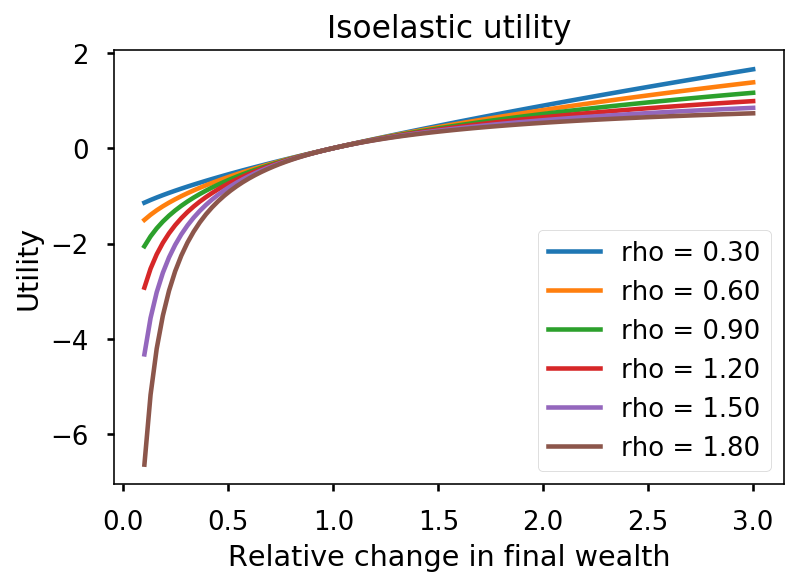
\includegraphics[width=0.7\linewidth]{Thesis/images/isoelastic}
		\caption{Изоэластичная функция полезности}
		\label{fig:isoelastic}	
	\end{figure}
\end{minipage}
\vspace{.5cm}

Это изоэластичная функция полезности. При $\rho=0$ функция полезности риск нейтральна, при $\rho \to \infty$ достигается абсолютное избегание риска. Для составления портфеля максимизируется её  матожидание:
\begin{equation}
\Eb[r_w]{U_\rho(r_w)} \to \max_w, \quad w>0,\quad \sum w = 1
\end{equation}
    % Вторая глава
\chapter{Практическое применение модели}
Понимание того, как будет работать модель на практике, важная часть исследовательской деятельности. На основе экспериментов можно будет давать практические рекомендации по подбору параметров, спецификации при использовании. Правильная постановка эксперимента позволит сравнить предложенный метод с бейзлайном.

\section{Описание данных}
\note{Этап создания алгоритмов}
Инфраструктура, созданная в компании предусматривает взаимодействие с широким кругом лиц, которые внештатно создают торговые стратегии, получая за это небольшое вознаграждение. При написании алгоритма можно:
\begin{enumerate}
	\item выбрать торгуемые активы
	\item задать периодичность, с которой работает алгоритм
	\item собирать любые статистики с предыдущих периодов
	\item произвольным образом реструктурировать портфель основываясь на прошлой информации
\end{enumerate}
Обладая навыками программирования на \texttt{Python}, можно написать любую стратегию, которая использует только рыночные данные. Алгоритмов огромное количество, более 700 000, большинство из этих алгоритмов написаны энтузиастами. В отличие от рыночных активов, которых ограниченное количество, алгоримов гораздо больше. Это открывает широкие возможности для применения портфельной теории для создания диверсифицированного портфеля.

\note{Этап селекции алгоритмов}
Тем не менее, применять портфельную теорию проблематично. Для такого количества временных рядов длина ряда слишком мала. Расчет даже ковариационной матрицы требует огромных вычислительных мощностей и памяти. Для решения этой проблемы существует этап предварительного отбора алгоритмов, этап селекции. В инфраструктуре разработана модель, которая выбирает наиболее стабильные из совокупности\footnote{Детали реализации защищены NDA}. После этого этапа остается около 150 торговых стратегий, которые и были использованы для тестирования модели динамики.

\section{Выбор спецификации модели}
Перед непосредственно оценкой спецификаций модели динамики доходностей, был проведен эмпирический анализ алгоритмов, отобранных после селекции. Основной его задачей было выяснить, какие предпосылки себя оправдывают и какая спецификация наиболее полно описывает распределение доходностей во времени. 

\begin{figure}[h]
	\centering
	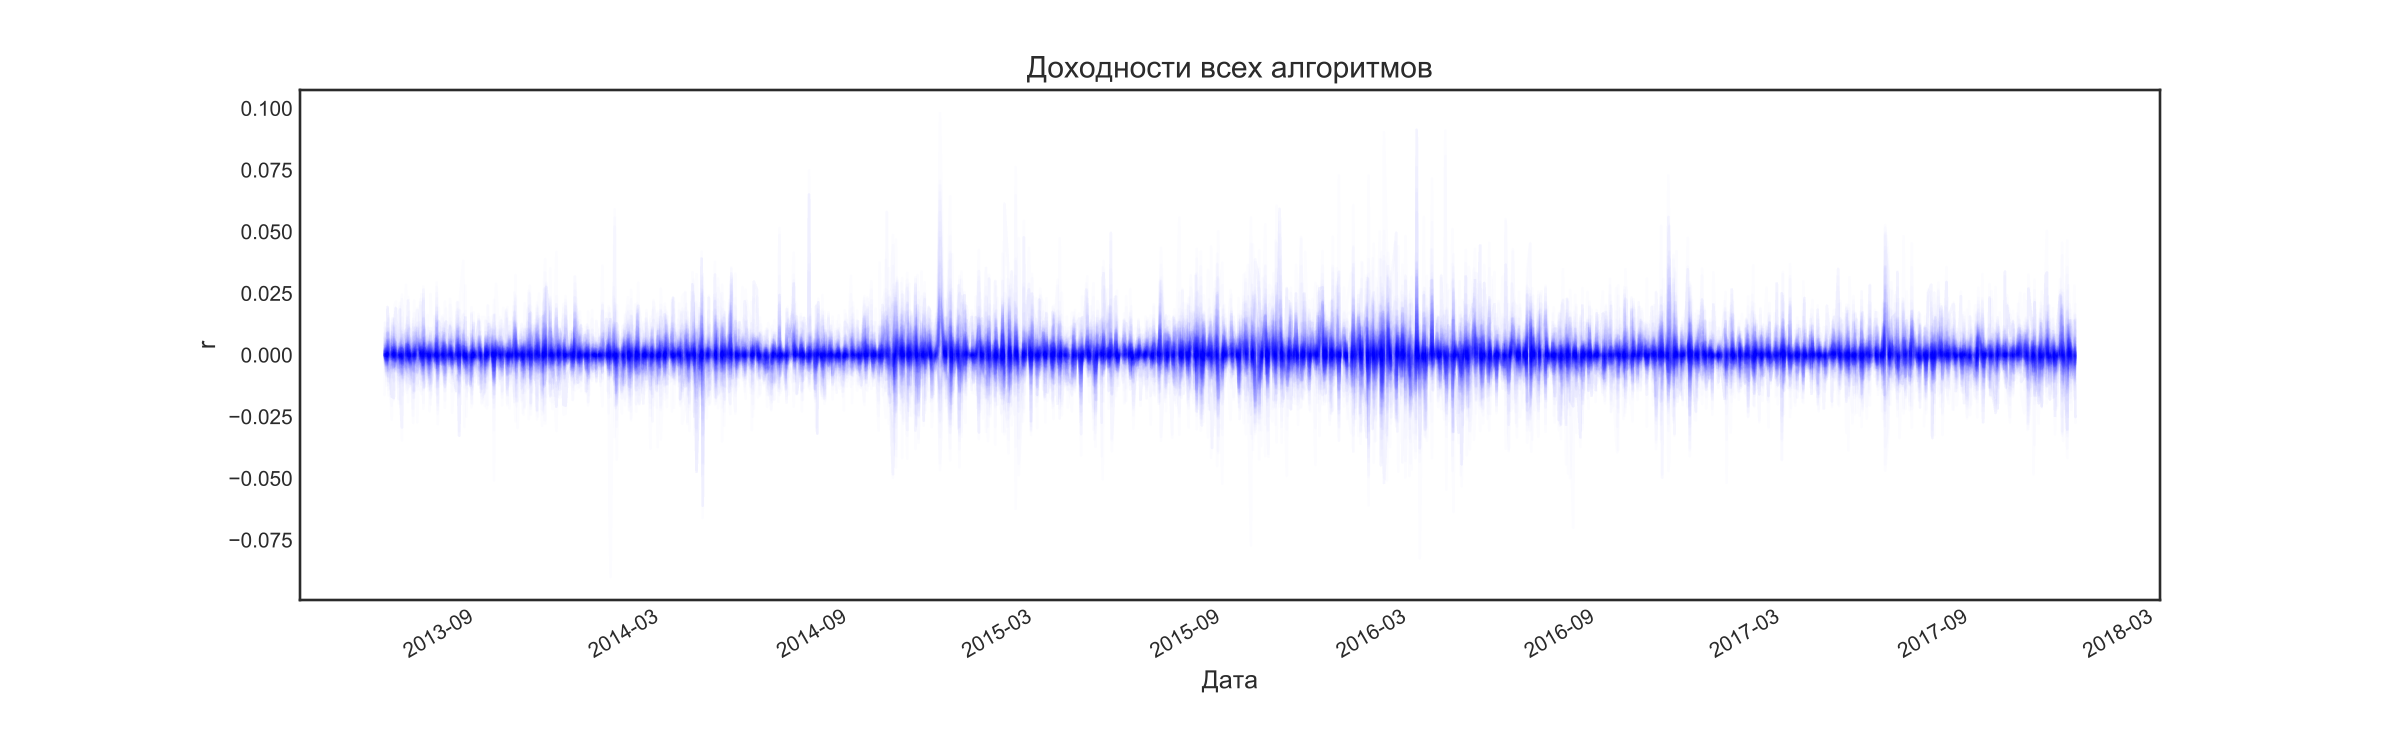
\includegraphics[width=\linewidth]{Thesis/images/returns-all}
	\caption{Доходности всех алгоритмов, на графике наблюдается непостоянная волатильность}
	\label{fig:allreturns}
\end{figure}

Гипотеза о непостоянстве волатильности находит свое подтверждение в графике распределения доходностей всех алгоритмов во времени (Рисунок \ref{fig:allreturns}). На нем видны периоды с высокой волатильностью. Более того, эффект наблюдается во многих алгоритмах в рамках одного периода.	

\begin{wrapfigure}{r}{.49\linewidth}
	\centering
	\includegraphics[width=\linewidth]{Thesis/images/returns-monthly}
	\caption{Распределение доходностей всех алгоритмов, сгруппированные по месяцам}
	\label{fig:monthlyreturns}
\end{wrapfigure}

Первичный анализ наличия сезонности в общем поведении алгоритмов не дал результатов: распределение доходностей, сгруппированных по месяцам выглядит однородно (Рисунок \ref{fig:monthlyreturns}).

\begin{figure}[h]
	\centering
	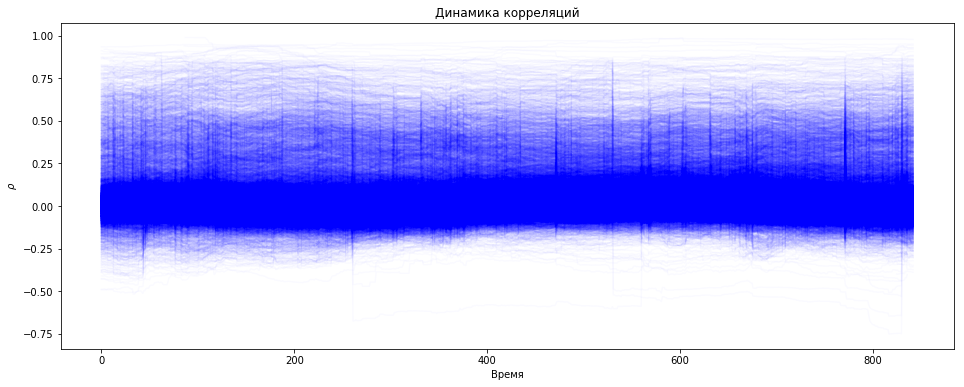
\includegraphics[width=\linewidth]{Thesis/images/correlations}
	\caption{График динамики корреляций между торговыми стратегиями. Попарные корреляции были посчитаны за период 2013-2017 с окном 300 дней. Не наблюдается существенного изменения корреляций за этот период.}
	\label{fig:correlations}
\end{figure}
Этап селекции имел важные последствия на спецификацию модели. Предположение о динамике корреляций оказалось не состоятельным (Рисунок \ref{fig:correlations}). В данных не наблюдается существенного изменения корреляций для большой группы торговых стратегий. Значительное количество траекторий значительно отдалены от нуля. Тем не менее, на основе этого графика сделать вывод о структуре ковариационной матрицы (блочная/плотная) нельзя. В сложившейся ситуации этот анализ избыточен, так как семейство моделей с плотной матрицей ковариации включает в себя подмножество тех, что имеют блочную структуру. 

Выводы, которые можно сделать на основе проведенного анализа:
\begin{itemize}
	\item присутствует стохастическая волатильность
	\item сезонность в данных отсутствует или незначительна
	\item корреляции относительно стабильны во времени
	\item большинство корреляций околонулевые
\end{itemize}

Основываясь на них остается сфокусироваться на двух спецификациях, которые не учитывают динамику корреляций:
\begin{itemize}
	\item модель без корреляций \eqref{eq:nocorr}
	\item модель со статичными корреляциями \eqref{eq:staticcorr}
\end{itemize}

Ковариционная матрица стабильна во времени, существуют негативные корреляции, много корреляций отличных от нуля, она имеет плотную структуру, которую невозможно учесть, используя блокдиагональную матрицу. Модель, учитывающая динамику корреляций, не подходит для моделирования стохастического процесса доходностей торговых стратегий. Более того, в экспериментах модель страдала от ряда проблем:
\begin{itemize}
	\item Долгая фаза адаптации ковариационной матрицы пропозал распределения
	\item Долгая сходимость марковской цепи (более 10000 итераций)
	\item Продолжительные расчеты для оценки модели (около 12 ч.)
	\item Модель не работала для моделирования динамики большой группы алгоритмов
\end{itemize}

\section{Постановка эксперимента и оценка модели}
\note{Описание поставленного эксперимента}
Для качественных выводов о работе предложенного метода составления портфеля недостаточно оценить одну модель на подвыборке алгоритмов, так как это может быть случайный успех или неудача. Для проведения эксперимента на реальных данных был использован метод бутстрэп \citep{grimshaw1995} и разделение выборки на обучающую и тестовую. 

\begin{itemize}
	\item Всего 4 года наблюдений
	\item Обучающая выборка -- первые два года
	\item Тестовая выборка -- последние два года
	\item Сгенерировано 400 выборок алгоритмов размера 20 из 150 без повторений
	\item Двумя методами: предложенным и по Марковицу, строятся портфели основываясь на данных обучающей выборки
	\item Считается критерий качества (коэффициент Шарпа) на тестовой выборке
\end{itemize}

\note{Параметры NUTS}
Для оценки апостериорных распределений параметров модели использовался зарекомендовавший себя алгоритм NUTS \citep{hoffman2011nuts}, при этом генерировалась выборка размера 3000 из этого распределения. Для оценки потребовались большие вычислительные мощности. Так, расчет модели на динамику 20-ти алгоритмов со статическими корреляциями \eqref{eq:staticcorr} занимает около 3х часов на 32х-ядерном сервере. Оценка модели без корреляций \eqref{eq:nocorr} занимает около получаса. 

\section{Сравнение метода с портфельной теорией Марковица}
\begin{figure}[t]
	\centering
	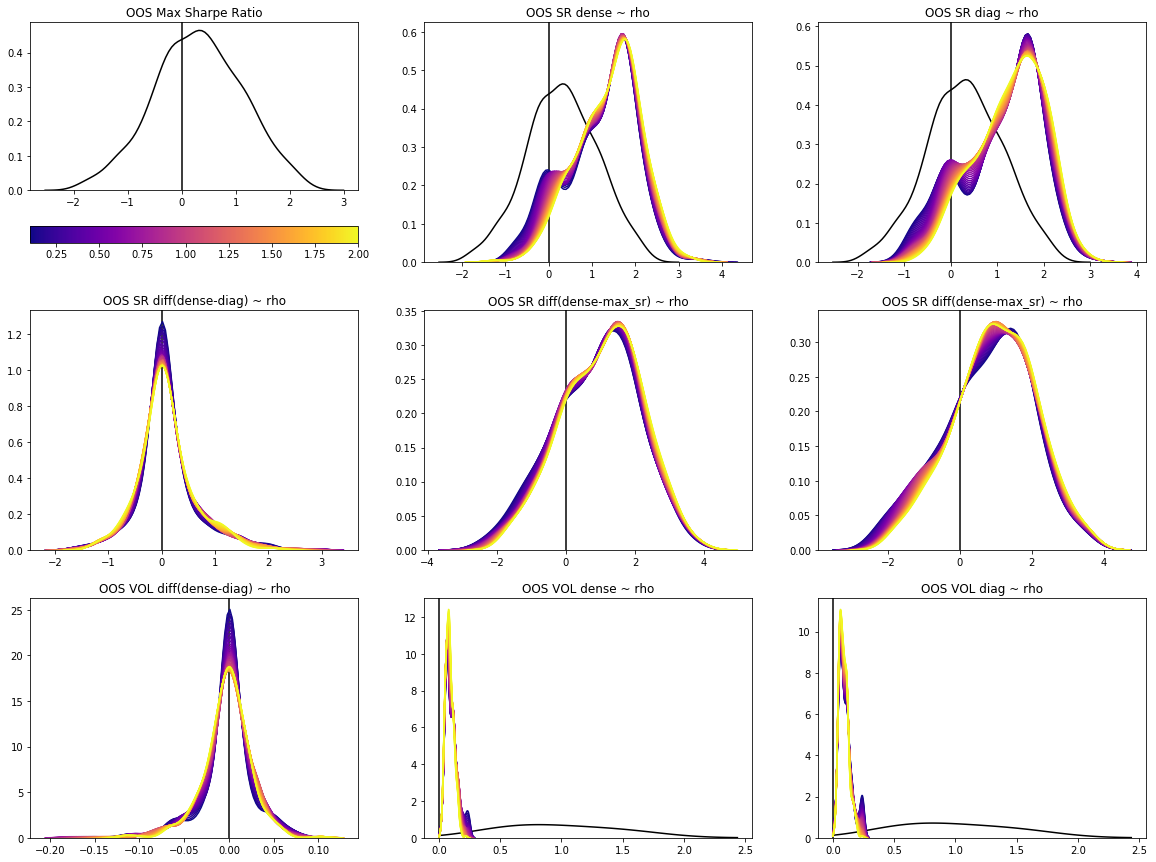
\includegraphics[width=\linewidth]{Thesis/images/performance}
	\caption{Сравнение коэффициента Шарпа на тестовой выборке байесовского (выделен цветом) и оптимального портфеля Марковица. Цветовая шкала означает значение параметра $\rho$ в функции полезности \eqref{eq:isoelastic}. Распределение коэффициента Шарпа на тестовом периоде находится значительно правее, что означает преимущество предложенного метода над ранее используемым аналогом}
	\label{fig:performance}
\end{figure}

\note{Описание и трактовка результатов}

Из экспериментов следует, что предложенный алгоритм более устойчив при обучении, обладает необходимой обобщающей способностью для улучшения качества портфеля по ряду показателей. В целом не важно, какую спецификацию модели выбирать: дополнительное моделирование корреляций не принесло большой пользы, разница волатильности и коэффициентов Шарпа между моделью \eqref{eq:staticcorr} и \eqref{eq:nocorr} имеет сконцентрированное в нуле распределение.

\begin{itemize}
	\item Коэффициент Шарпа: в 70\% случайно выбранных портфелях коэффициент Шарпа больше полученного методом Марковица
	\item Дисперсия получаемого портфеля новым способом ниже
	\item Моделирование корреляций не дает существенного преимущества перед моделью без них
\end{itemize}

   % Третья глава
\chapter*{Заключение}
\addcontentsline{toc}{chapter}{Заключение}

В ходе проведенного исследования решены следующие задачи:
\begin{enumerate}
	\item Предложена общая схема моделирования динамики торговых стратегий, которая учитывает особенности, связанные с их доходностями. Результаты исследования включают в себя реализацию трех спецификаций модели с учетом, без учета динамики корреляций и упрощенная -- без корреляций. Для оценки модели динамики корреляций предложена модификация базового метода DECO с использованием гауссовского процесса

	\item Все три спецификации модели динамики доходностей торговых стратегий были реализованы на языке \texttt{Python} с использованием специализированных библиотек для байесовского моделирования
	
	\item Была реализована процедура составления портфеля торговых стратегий методом монте--карло

	\item Эмпирический анализ позволяет сделать вывод о непостоянстве волатильности, и постоянстве корреляций доходностей торговых стратегий

	\item Проведенные эксперименты показали практическую значимость предложенного подхода для использования его в качестве инструмента для составления портфеля торговых стратегий.
	Портфель, основанный на предложенной модели оказывается эффективнее модели Марковица по ряду критериев (имеет большую обобщающую способность, более высокое Шарпа на экзаменационной выборке). Оптимизация матожидания полезности инвестора позволяет получить более устойчивый во времени портфель.

\end{enumerate}

Проведенное исследование подтверждает целесообразность использования байесовских методов в формировании портфеля торговых стратегий. Такой подход позволяет учесть априорные знания о модели. Портфель, построенный на симуляциях из нее, получается более устойчивым во времени и, как следствие, более доходным на экзаменационном периоде.

      % Заключение
\include{Thesis/references}      % Список литературы
\include{Thesis/appendix}        % Приложения

\end{document}
